% Slide 4 — QR as a Task DAG (Updated with simplified alertblock bullets)
\begin{frame}{Problem Formulation: QR as a Task DAG}
	
	\pause 
	
	% Use [T] to top-align the columns for better control over vertical space
	\begin{columns}[c,onlytextwidth] 
		% ---------- LEFT: Content drastically condensed into a single block ----------
		\column{0.60\textwidth}
		\begin{block}{Task \& Dependency Model}
		  The QR algorithm is modeled as a DAG of tasks, $T_{i,j}$:
		  \begin{itemize}\setlength{\itemsep}{3pt} % Tighter item spacing
		    \item \textbf{Pivot Task ($T_{i,i}$):} Runs \texttt{update\_pivot\_row}.
		    \item \textbf{Update Task ($T_{i,j}, j>i$):} Runs \texttt{update\_trailing\_non\_pivot\_row}. % FIXED: Changed &gt; to > for LaTeX compatibility
		    \item \textbf{Dependencies:} A task $T_{i,j}$ can only run after its parents, \textbf{$T_{i,i}$} (pivot) and \textbf{$T_{i-1,j}$} (previous row), are complete.
		  \end{itemize}
		\end{block}
	
		\pause 
		\begin{alertblock}{Scheduling Goal}
		  \begin{itemize}\setlength{\itemsep}{3pt} % Keep bullets tight to fit page
		    \item Execute the task DAG in parallel.
		    \item Respect all task dependencies.
		    %\item Avoid the overhead caused by global synchronization barriers.
		  \end{itemize}
		\end{alertblock}
	
		% ---- Right: TaskGraph figure with adjusted scale and caption ----		
		\column{0.40\textwidth}
		\centering
		\definecolor{lightblue}{RGB}{173, 216, 230}
		
		% --- Further reduced scale to guarantee fit ---
		\pause 
		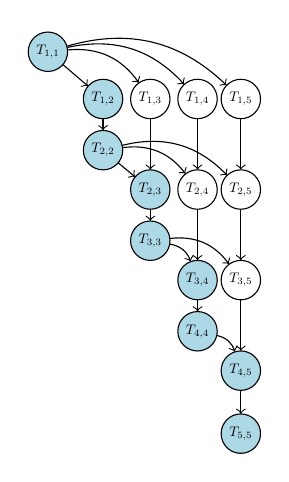
\begin{tikzpicture}[node distance=1cm and 0.5cm, scale=0.5, transform shape]
			% Nodes - Row 1
			\node[draw, circle, fill=lightblue] (T11) at (0,0) {$T_{1,1}$};
			\node[draw, circle, fill=lightblue] (T12) at (1.4,-1.2) {$T_{1,2}$};
			\node[draw, circle] (T13) at (2.6,-1.2) {$T_{1,3}$};
			\node[draw, circle] (T14) at (3.8,-1.2) {$T_{1,4}$};
			\node[draw, circle] (T15) at (4.9,-1.2) {$T_{1,5}$};
			
			% Nodes - Row 2
			\node[draw, circle, fill=lightblue] (T22) at (1.4,-2.5) {$T_{2,2}$};
			\node[draw, circle, fill=lightblue] (T23) at (2.6,-3.5) {$T_{2,3}$};
			\node[draw, circle] (T24) at (3.8,-3.5) {$T_{2,4}$};
			\node[draw, circle] (T25) at (4.9,-3.5) {$T_{2,5}$};
			
			% Nodes - Row 3
			\node[draw, circle, fill=lightblue] (T33) at (2.6,-4.8) {$T_{3,3}$};
			\node[draw, circle, fill=lightblue] (T34) at (3.8,-5.8) {$T_{3,4}$};
			\node[draw, circle] (T35) at (4.9,-5.8) {$T_{3,5}$};
			
			% Nodes - Row 4
			\node[draw, circle, fill=lightblue] (T44) at (3.8,-7.1) {$T_{4,4}$};
			\node[draw, circle, fill=lightblue] (T45) at (4.9,-8.1) {$T_{4,5}$};
			
			% Nodes - Row 5
			\node[draw, circle, fill=lightblue] (T55) at (4.9,-9.7) {$T_{5,5}$};
			
			% Edges (condensed to save space in the .tex file)
			\draw[->] (T11) -- (T12); \draw[->] (T12) -- (T22); \draw[->] (T13) -- (T23);
			\draw[->] (T14) -- (T24); \draw[->] (T15) -- (T25); \draw[->, bend left] (T11) to (T13);
			\draw[->, bend left] (T11) to (T14); \draw[->, bend left] (T11) to (T15);
			\draw[->] (T22) -- (T23); \draw[->] (T24) -- (T34); \draw[->] (T25) -- (T35);
			\draw[->, bend left] (T22) to (T24); \draw[->, bend left] (T22) to (T25);
			\draw[->] (T23) -- (T33); \draw[->, bend left] (T33) to (T34); \draw[->, bend left] (T33) to (T35);
			\draw[->] (T34) -- (T44); \draw[->] (T35) -- (T45); \draw[->, bend left] (T44) to (T45);
			\draw[->] (T45) -- (T55);
		\end{tikzpicture}
		
		% --- Added the requested figure caption ---
		\vspace{1mm}
		{\scriptsize \emph{TaskGraph for Triangular System}}
	
	\end{columns}
\end{frame}
